
\documentclass{beamer}


\usetheme{Warsaw}
\usecolortheme{crane}


\title{Regression Techniques}
\subtitle{Probability and Statistics for Engineers and Scientists}
\author{Steve Mazza}
\institute[Naval Postgraduate School]
{ 
    Naval Postgraduate School \\
    Monterey, CA \\
    
\includegraphics[height=3cm]{images/NPS_logo.jpg}
}
\date {SE3030, Winter/2014 \\ Quantitative Methods of Systems Engineering}
\subject{Quantitative Methods of Systems Engineering}


\begin{document}

\frame{\titlepage}


\frame{{Introduction}
  \begin{columns}[c]
    \column{.4\textwidth}
      Regression uses selected values of $x$ and observed values of $y$ in order to predict the most probable value of $y$ for any value of $x$.
    \column{.6\textwidth}
    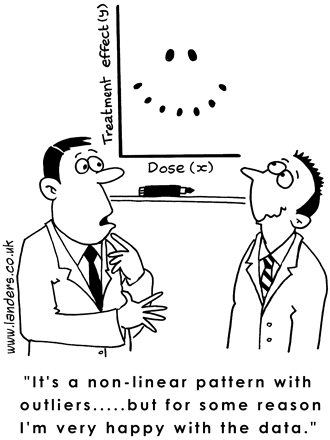
\includegraphics[scale=0.4]{images/Regression-Cartoon.png}
  \end{columns}
}


\frame{{Simple Linear Regression}
  %TODO: Enter reminder. (mazzas) Fri Feb 21 09:21:37 2014
}


\frame{{Multiple Linear Regression}
  %TODO: Enter reminder. (mazzas) Fri Feb 21 09:21:37 2014
}


\frame{{Questions?}
	\begin{center}
		
\includegraphics[width=.7\textwidth]{images/fin.png}
	\end{center}
}

\end{document}
